\documentclass[]{article}
\usepackage{lmodern}
\usepackage{amssymb,amsmath}
\usepackage{ifxetex,ifluatex}
\usepackage{fixltx2e} % provides \textsubscript
\ifnum 0\ifxetex 1\fi\ifluatex 1\fi=0 % if pdftex
  \usepackage[T1]{fontenc}
  \usepackage[utf8]{inputenc}
\else % if luatex or xelatex
  \ifxetex
    \usepackage{mathspec}
  \else
    \usepackage{fontspec}
  \fi
  \defaultfontfeatures{Ligatures=TeX,Scale=MatchLowercase}
\fi
% use upquote if available, for straight quotes in verbatim environments
\IfFileExists{upquote.sty}{\usepackage{upquote}}{}
% use microtype if available
\IfFileExists{microtype.sty}{%
\usepackage{microtype}
\UseMicrotypeSet[protrusion]{basicmath} % disable protrusion for tt fonts
}{}
\usepackage[margin=1in]{geometry}
\usepackage{hyperref}
\hypersetup{unicode=true,
            pdftitle={Matching estimators and flooding},
            pdfauthor={Leon Stirk-Wang},
            pdfborder={0 0 0},
            breaklinks=true}
\urlstyle{same}  % don't use monospace font for urls
\usepackage{graphicx,grffile}
\makeatletter
\def\maxwidth{\ifdim\Gin@nat@width>\linewidth\linewidth\else\Gin@nat@width\fi}
\def\maxheight{\ifdim\Gin@nat@height>\textheight\textheight\else\Gin@nat@height\fi}
\makeatother
% Scale images if necessary, so that they will not overflow the page
% margins by default, and it is still possible to overwrite the defaults
% using explicit options in \includegraphics[width, height, ...]{}
\setkeys{Gin}{width=\maxwidth,height=\maxheight,keepaspectratio}
\IfFileExists{parskip.sty}{%
\usepackage{parskip}
}{% else
\setlength{\parindent}{0pt}
\setlength{\parskip}{6pt plus 2pt minus 1pt}
}
\setlength{\emergencystretch}{3em}  % prevent overfull lines
\providecommand{\tightlist}{%
  \setlength{\itemsep}{0pt}\setlength{\parskip}{0pt}}
\setcounter{secnumdepth}{0}
% Redefines (sub)paragraphs to behave more like sections
\ifx\paragraph\undefined\else
\let\oldparagraph\paragraph
\renewcommand{\paragraph}[1]{\oldparagraph{#1}\mbox{}}
\fi
\ifx\subparagraph\undefined\else
\let\oldsubparagraph\subparagraph
\renewcommand{\subparagraph}[1]{\oldsubparagraph{#1}\mbox{}}
\fi

%%% Use protect on footnotes to avoid problems with footnotes in titles
\let\rmarkdownfootnote\footnote%
\def\footnote{\protect\rmarkdownfootnote}

%%% Change title format to be more compact
\usepackage{titling}

% Create subtitle command for use in maketitle
\providecommand{\subtitle}[1]{
  \posttitle{
    \begin{center}\large#1\end{center}
    }
}

\setlength{\droptitle}{-2em}

  \title{Matching estimators and flooding}
    \pretitle{\vspace{\droptitle}\centering\huge}
  \posttitle{\par}
    \author{Leon Stirk-Wang}
    \preauthor{\centering\large\emph}
  \postauthor{\par}
      \predate{\centering\large\emph}
  \postdate{\par}
    \date{7/31/2019}


\begin{document}
\maketitle

\subsection{Intro}\label{intro}

On the 4th of June 2015 South Dunedin experienced a flooding event. At
the time, news outlets reported that 400 emergency call were made
regarding the flooding, and that the army, firefighters, and volunteers
had sandbagged around 100 houses. Later measurements of surface ponding
depth indicated a significant amount of ponding of up to 30 centimetres
in depth over the approximately 2.5 square kilometres that were worst
affected. A smaller number of measurements were significantly higher
with some measurements in the range of 50 to 60 centimetres of ponding
above ground level.

The effects of the weather event that that precipitated the flooding
event were not limited to South Dunedin. The heavy rain caused slips
that necessitated the closure of roads. Several schools were evacuated
and there was a significant threat to property in the surrounding
semi-rural areas built on the floodplain of the Taieri river. However,
it is specifically the flooding in South Dunedin, rather than the more
widespread effects of the severe weather event, that is of primary
interest in this paper.

The analysis presented in this paper examines the Dunedin real-estate
market and produces estimates of the impact of the 2015 flooding event
on residential property prices. The intention is to provide an
understanding of the market response to natural hazard risk and changing
information about those risks in the face of a destructive event.

\begin{figure}

{\centering 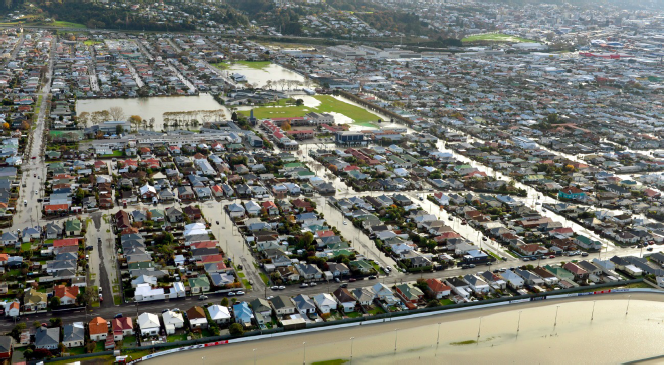
\includegraphics[width=0.5\linewidth]{../images/flooding_4June2015} 

}

\caption{...}\label{fig:unnamed-chunk-1}
\end{figure}

Dunedin is of special interest with respect to flood risks. It is a city
located at the southern end of the South Island of New Zealand. It is
the principal city of the Otago region and the second most populous city
in the South Island. As of June 2018 the urban area was estimated to be
home to around 122,000 people.

Dunedin has around 2700 residences located within 50 centimetres of the
spring high-tide mark. This is higher than any other city in New Zealand
and represents a not insignificant proportion of the residential housing
stock. These houses face the most immediate risk of inundation due to
sea-level rise. The threat of inundation is not one that can be
considered in isolation. Rising average global temperatures will not
only increase the ground-water level via sea-level rise but will
increase the frequency and severity of weather events. The combination
of these effects will compound the risks to low-lying properties. The
most-recent experience of flooding events are a sobering reminder of
this. Most of the properties identified as being at the greatest risk
are located on the South Dunedin plain.

\begin{center}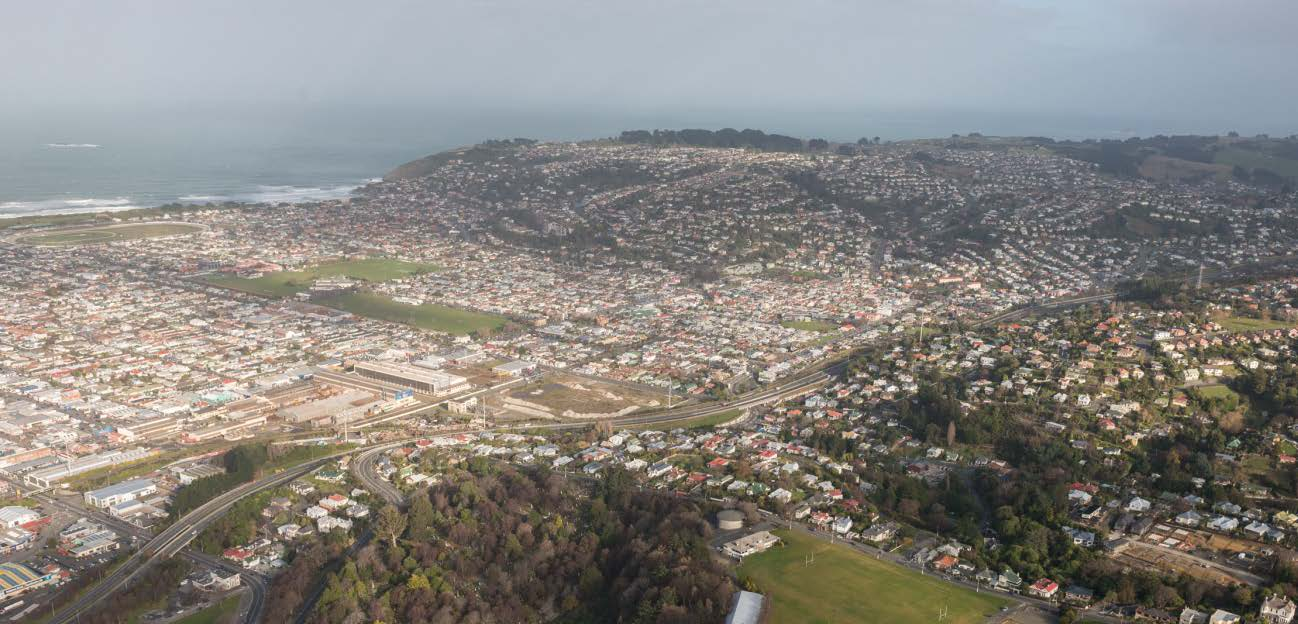
\includegraphics[width=0.5\linewidth]{../images/south_dunedin_aerial_1} \end{center}

\begin{center}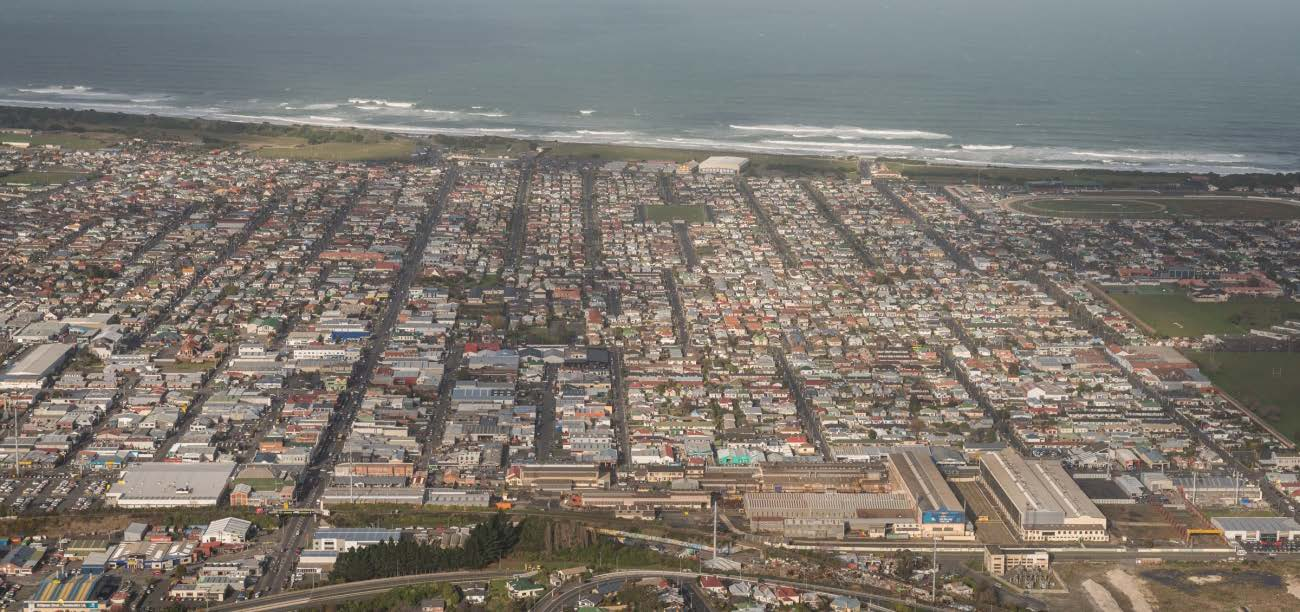
\includegraphics[width=0.5\linewidth]{../images/south_dunedin_aerial_2} \end{center}

\begin{center}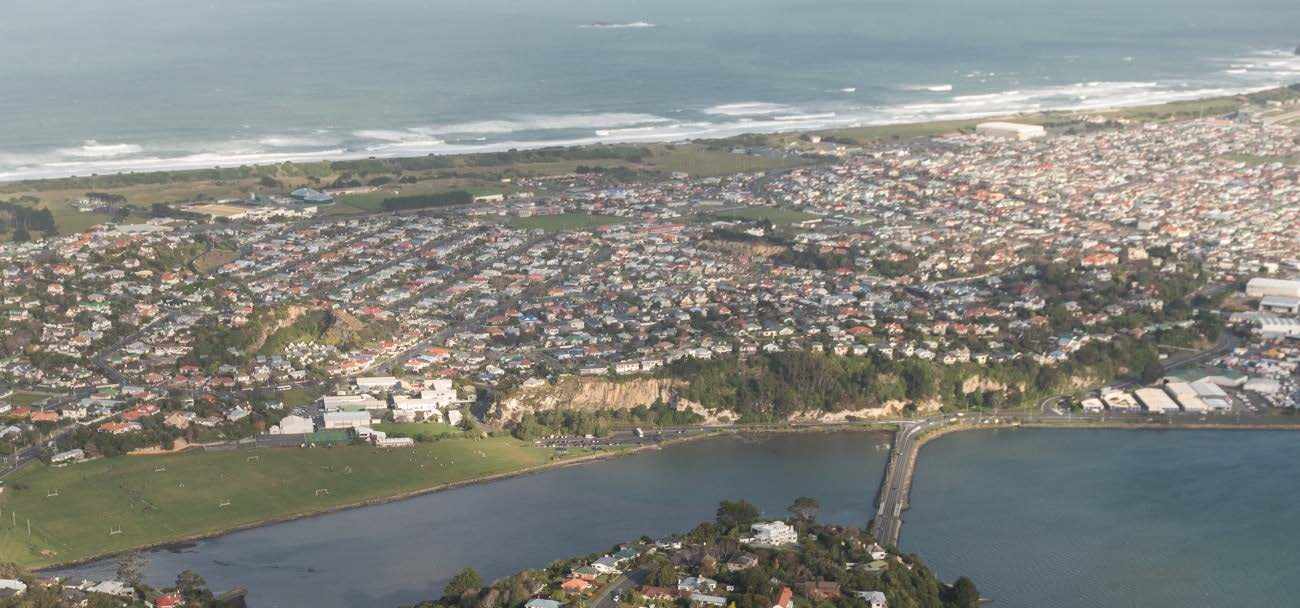
\includegraphics[width=0.5\linewidth]{../images/south_dunedin_aerial_3} \end{center}

Geologically, the South Dunedin plain was formed in the last glacial
period when the sea-level was significantly lower than it is now.
Beneath the plain is a valley of volcanic bedrock. During this glacial
period the catchment area that is now the Otago harbour drained through
this valley out toward the coast depositing sands, silts, and gravels
along the valley bed. As the sea rose to its current level, these sands,
silts, and gravels consolidated in the valley to form a relatively flat
plain. Prior to European settlement, the area of land on this plain that
was suitable to be built upon was considerably smaller than it is today.
The spring-high tide mark on both the harbour side and to the south
extended significantly further inland than the present day coastline.
There were large areas of wetland in what are now the suburbs of
Musselburgh and St Kilda that drained into a saltwater lagoon inland of
the modern high tide mark.

\begin{center}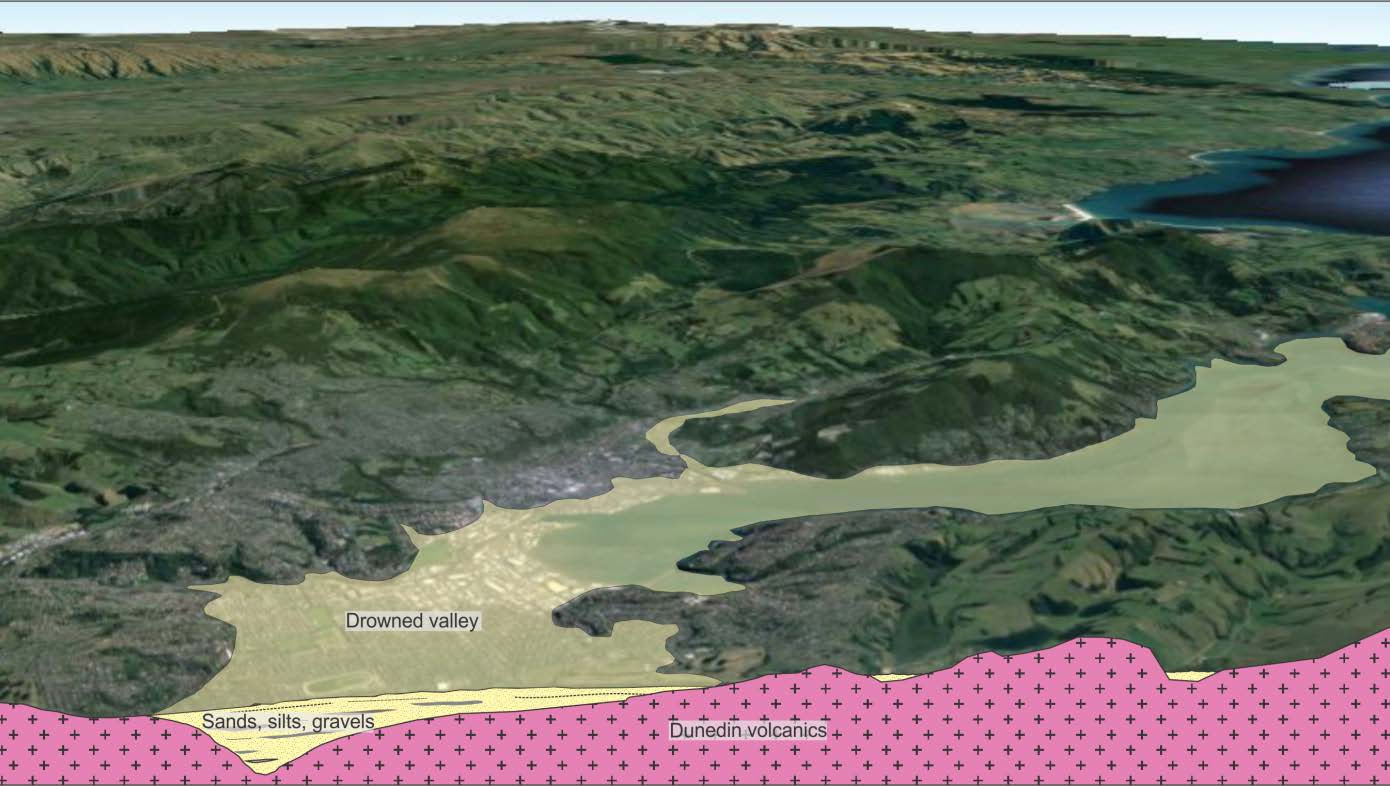
\includegraphics[width=0.5\linewidth]{../images/sd_historical_1} \end{center}

\begin{center}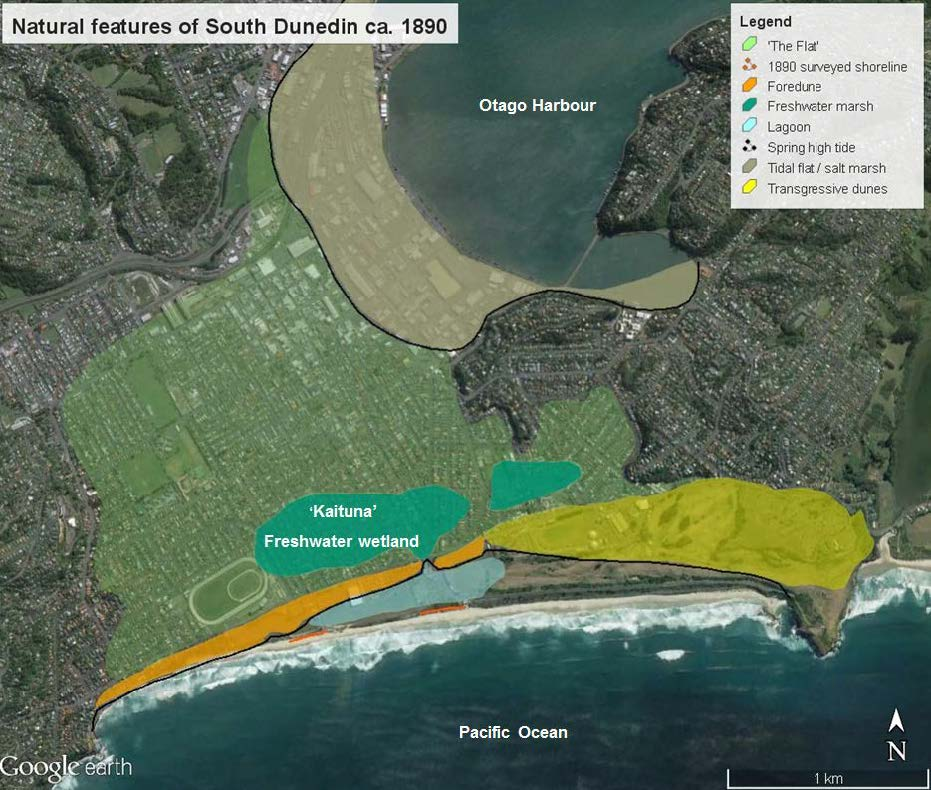
\includegraphics[width=0.5\linewidth]{../images/sd_historical_2} \end{center}

\begin{center}
\includegraphics[width=0.5\linewidth]{../images/sd_historical_3} \end{center}

The mid to late 19th century saw a period of rapid settlement by
Europeans. The demand for dry land saw the settlers undertake land
reclamation activities. This largely consisted of filling in wet,
marshy, or low areas with any available infill material. This included
sand that was mined from the nearby coastal dunes. Although early
reclamation efforts centred around the shoreline of the harbour, these
eventually extended further south to what are modern day residential
areas. Early reclamation efforts reflect the level of the groundwater at
the time which was up to 17cm lower than the present day level.
Subsequent infilling in the 1960's and 70's of the harbour-side
waterfront with dredge spoil raised the ground level in the area between
Portsmouth Drive and Andersons Bay Road to a sufficient degree that the
present-day groundwater level is not problematic. However, the ground
level of the majority of the South Dunedin plain, comprised mostly of
residential properties, remains unchanged since the reclamation
activities of the mid to late 1800's.

\begin{center}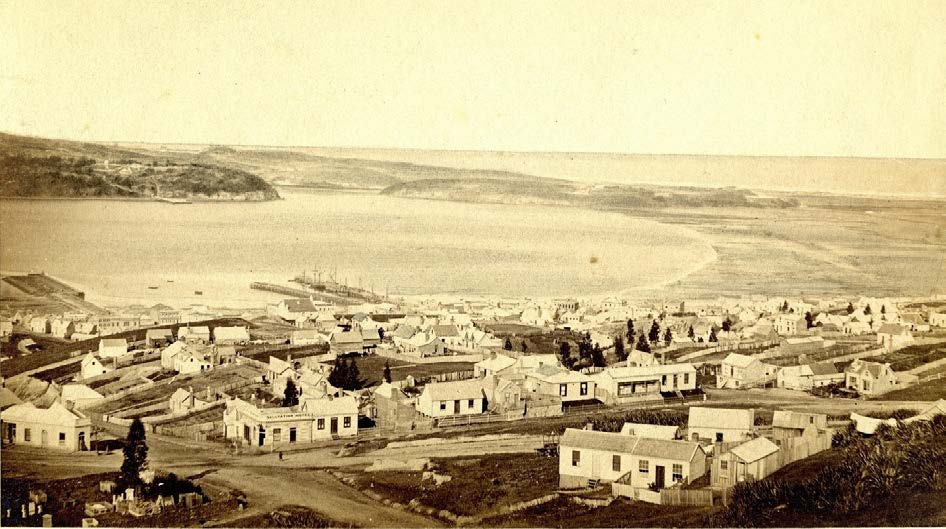
\includegraphics[width=0.5\linewidth]{../images/sd_historical_4} \end{center}

\begin{center}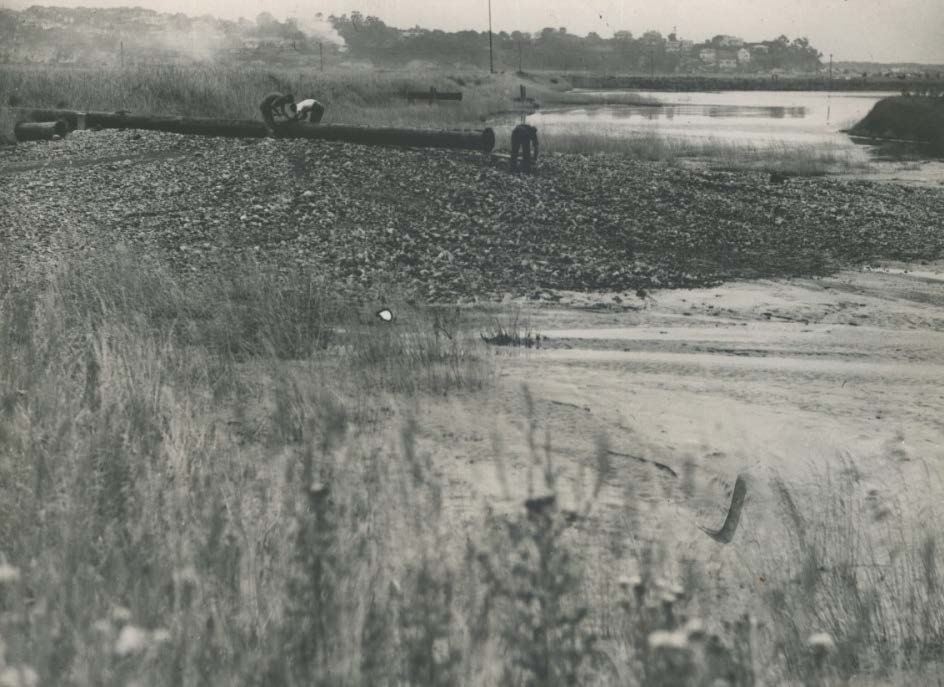
\includegraphics[width=0.5\linewidth]{../images/sd_historical_5} \end{center}

\begin{center}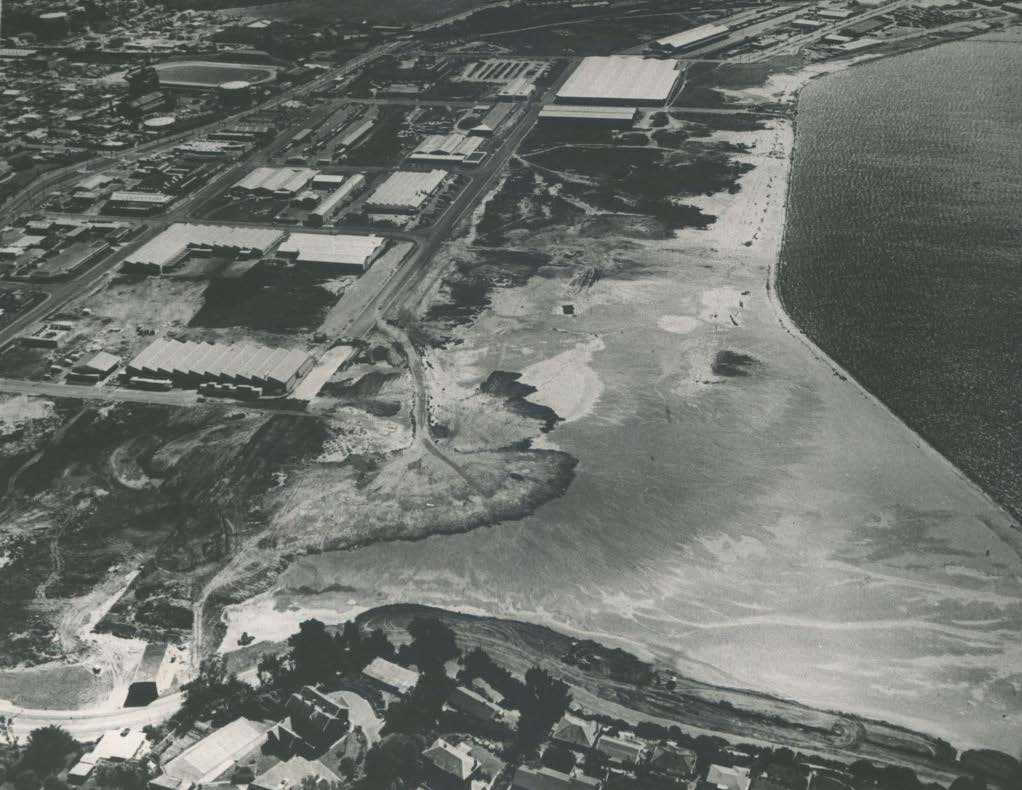
\includegraphics[width=0.5\linewidth]{../images/sd_historical_6} \end{center}

Today, South Dunedin plain has a mix of residential commercial and
industrial zoning although the bulk of the plain, and indeed the areas
worst affected were primarily residential. For administrative purposes
the plain is split into several area units. Area units (or `census area
units') are a standard, intermediate administrative unit used by local
and state government institutions that represent what might commonly be
referred to as a `suburb'. Each area unit is comprised of even smaller
administrative units known as meshblocks. Meshblocks are the smallest
administrative unit of aggregation and are typically comprised of a
couple of dozen houses. Commonly the boundaries will run along roads.
These might be thought of as small `neigbourhoods' but this is perhaps a
less than ideal analogue.

During the June 2015 flooding event only part of the South Dunedin plain
was seriously affected. Other areas experienced little to no inundation.
This is despite the fact that almost the entirety of the plain has an
elevation fairly uniformly within 1 metre of the mean sea-level. Here
the mean-sea level might be considered a reasonable if imperfect proxy
for the groundwater level. And, at least anecdotally, the uniform
`low-lyingness' of the plain as a whole is a proxy for the level of
flood risk as might be perceived by real-estate market participants.
That is, we might reasonably expect that prospective purchasers of
residential properties on the South Dunedin plain to consider the flood
risk to all properties with the same elevation above the mean sea-level
to be approximately equal either over the long term or in the absence of
any additional information (such as the kind provided by a flooding
event).

\begin{center}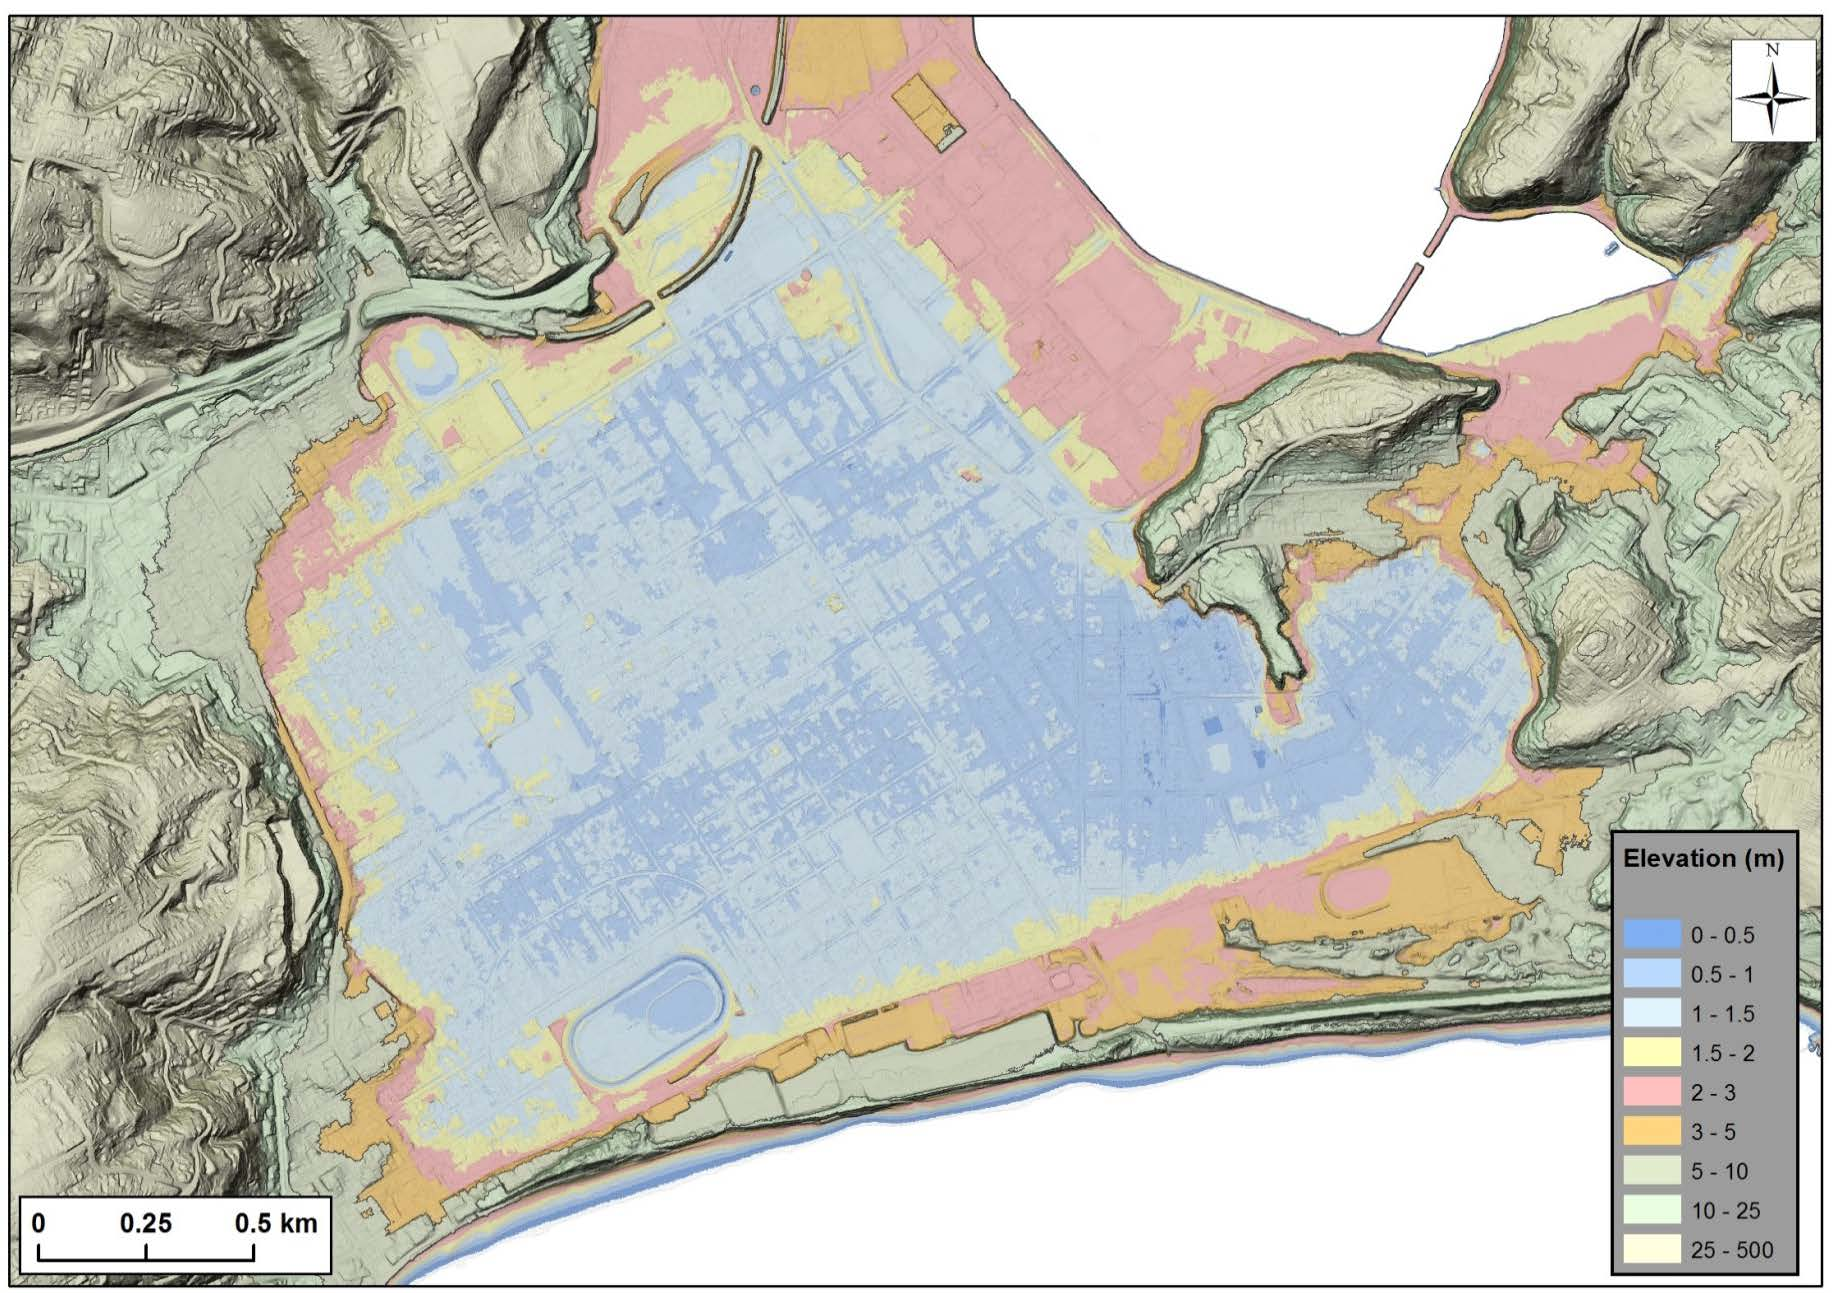
\includegraphics[width=0.5\linewidth]{../images/sd_elevation_1} \end{center}

This expectation, coupled with the non-uniform distribution of
inundation resulting from the June 2015 flood forms the basis for
understanding the results in this analysis as being those of a `natural
experiment'. Specifically, this analysis presents the results of three
questions asked of the natural experiment. Those questions are as
follows:

\begin{quote}
\emph{(1)} How did the real-estate market in Dunedin price flood risks
prior to the June 2015 flood?
\end{quote}

\begin{quote}
\emph{(2)} Did the price of those risks change in response to the flood?
\end{quote}

\begin{quote}
\emph{(3)} Did the spatial distribution of flood-risk prices change in
response to the flood?
\end{quote}

Further, this paper makes one contribution. That is, to show the
magnitude to which the estimation of these results is model dependent.
At each stage of the analysis, this paper will compare the results of
standard regression methods with those of `matching estimators'.
Matching estimators are an increasingly common technique used for causal
inference in observational studies of treatment effects. Simply put,
they are a way of matching treated and non-treated units of observation
based on their observed characteristics in order to improve estimates of
the causal effect of the treatment. The intention is to replicate as
closely as possible the conditions of a randomised controlled experiment
given the limitations of observational data. The benefit being that the
regression is required to do less `work' when estimating the effect of
the treatment. The coefficients estimated in the regression are
therefore less sensitive to model misspecification.

To say that a greater degree of model dependence in the unmatched
sample, in fact, over or under estimates the true effect of perceived
flood risk requires an understanding of the specific data generating
process. This paper attempts to validate matching as a method of
improving the performance of the model with respect to this data set. We
use effect-plus-partial-residual plots to visually identify the source
of differences in coefficient estimates produced by the matched and
unmatched samples.

All of the above questions are addressed in the substantive portion of
this paper with each building on the results of the last. That is, the
question as to the whether there is a change in the spatial distribution
of the `flood discount' is premised on there being a change in the
`flood discount' as a result of the 2015 flood event. In turn, the
ability to perceive a change in the flood discount requires a baseline
measurement of the existing price of flood risk on the South Dunedin
plain prior to the flood. Because it is the changes in relative
flood-risk price (with respect to location) that are of interest, a
natural modelling choice is the difference-in-differences (DiD)
approach. The analysis of the final question posed above is presented as
the results of an (incomplete) difference-in-difference-in-differences
regression. The specific details of the modelling will be explained in
further detail in the substantive portion of the paper.

\subsection{Some brief comments on
approach}\label{some-brief-comments-on-approach}

The analysis is carried out on a dataset comprised of all residential
property transactions occurring in the period January 2000 to September
2018. The unit of observation is a single transaction on a residential
property. The same property can therefore appear multiple times in the
data set if it has changed hands more than once in the sample period.

With respect to the three questions above, this paper tests for the
effect of the flood event, and the effect of location. This paper
characterises these as a set of binary variables, or `treatments'. The
flood event is a treatment with respect to the dimension of time. A
transaction occuring before the flood takes the value 0, a transaction
occuring after the flood takes the value 1.

\$\$

after\_flood = \left \{

\begin{array}{c c}
  0: & before flood \\
  1: & after flood \\
\end{array}

\right \}

\$\$

The location of properties can be thought of as a spatial treatment.
This paper considers four categories of location. The first category are
transactions on properties that would not be considered particularly
prone to flooding. Given the geographic history of Dunedin summarised
briefly above, this was defined as all those properties which did not
lie on the South Dunedin plain. For most of the models considered in
this paper, this is the `control' group. The second locational category
is defined as the transactions on properties which might have been
considered at risk of flooding (prior to the flood). This is defined as
the set of properties on the South Dunedin plain (broadly, the
complement of the first group).

The paper further decomposes this second category into two subsets that
are also considered `treatment' groups. the first of these is the set of
properties within the South Dunedin plain that, in fact, experienced
some significant inundation in the June 2015 flood. The other group is
the complement of the first, the properties which are located on the
South Dunedin plain but did not experience inundation.

There were no properties located outside the South Dunedin plain that
experienced inundation. For the purpose of this study there are three
unique (non-intersecting) groups that will be referred to as the:
`flooded' (located on the South Dunedin plain and experienced
inundation), `not flooded' (on the South Dunedin plain and did not
experience inundation), and `not flood prone' (outside the South Dunedin
plain) groups. What will be referred to as the flood prone group
(located on the South Dunedin plain) is simply the union of the sets of
`flooded' and `not flooded' properties.

In general, then, the independent variables of interest are some
combination of the flood-related treatments (with respect to time or
location). And the response variable is, of course, price.

The gold standard in experimental design, whenever a researcher is
interested in the causal effects of treatments, is the randomised
control trial. A randomised contol trial is an experimental design
method where the researcher collects a random sample of units, and
randomly assigns each to either the treatment or control group. It is
generally accepted that the effect of the treatment that is subsequently
observed is a causal one. The core principle is that by randomising the
treatment across the sample, the researcher will, by the law of large
numbers, have eliminated any correlation between the treatment and
either observed or unobserved characteristics across the treatment and
control groups.

In ideal circumstances, the randomisation of units to the treatment and
control groups will control for other variables so a simple difference
in means test will suffice to determine the causal effect of the
treatment. A more detailed discussion of randomised control trials
appears in the substantive conceptual section. Suffice it to say for now
that randomised control trials under ideal conditions reduce, to the
point of elimination, the burden of model specification.

The randomised control trial design however, requires the ability to
randomly assign units of observation to the treatment and control groups
over a given sample. Unfortunately, outside of a laboratory environment,
it is unusual for observational data (of the sort used in econometric
studies) to satisfy this requirement. The assignment of units to
treatment or control groups is usually outside of the control of the
researcher. And even in cases where the data can be thought of as a
`natural experiment' the treatment is usually less than completely
random.

Without the ability to design a randomised control experiment. The
researcher makes use of other tools to determine causality. Arguably the
most widely used of these is some form of least squares regression. By
controlling for the variation in the response variable associated with
variations in independent variables that are not of interest, the
researcher can isolate the effect of the independent variable of
interest.

It is well established that this kind of analysis is prone to error. The
source of error that this paper is primarily concerned with is model
misspecification error. Model misspecification error can arise where
there is misspecified functional form. For example, unmodelled
interactions between observed characteristics, or assuming linearity in
a non-linear parameter. Model misspecification might also be thought of
as error due to unmodelled and, therefore, presumably unobserved
variables.

Matching is a process by which the researcher can (imperfectly) simulate
the design of a randomised control trial with observational data.

reduce imbalance in the distributions of characteristics across
treatment groups in the sample. This paper will refer to this as `sample
imbalance reduction' for the sake of brevity. Reduction (to the point of
elimination) of sample imbalance is the objective of the design of the
randomised control trial.

One of the main functions of this paper is to understand the the effect
of matching on estimates produced using fairly conventional econometric
methods.

\subsection{A brief discussion of
results}\label{a-brief-discussion-of-results}

Prior to the June 2015 floods the market does not appear to price
flood-risks in a way that is statistically detectable when comparing the
low-lying South Dunedin plain to the remainder of Dunedin. A hedonic
regression specification estimating the price effect of being located on
the South Dunedin plain is carried out over the 3 year period leading up
to the flood event. In the period prior to the flood both matched and
unmatched sample estimates produce results camparably close to null.

A regression with the same specification is carried out over the three
year period following the flood event. After the flood the unmatched
regression estimates a highly significant 4.15\% discount associated
with the South Dunedin plain compared with the rest of Dunedin. The
matched sample regressions are more circumspect with respect to the size
and significance of the estimated discount. They estimate around a 2.1\%
discount associated with being low-lying with a mean level of
significance of 6.3\%. This implies that the June 2015 flood provided an
impetus for the market to re-evaluate the pricing of flood-risks on the
South Dunedin plain.

The fact that a discount appears to be associated with the flood event
invites the application of a differences-in-differences specification to
estimate the effect of the flood event in the South Dunedin plain. That
is, the interaction of the effect of the information provided by the
flood event (i.e.~a binary variable seperating transactions occuring
before the flood and after the flood) with a location `treatment'.

Further, the extent of the flood itself provides the market with
additional information about the relative flood risk of properties
located on different parts of the South Dunedin plain. That is, flooding
only occurred in a portion of the plain. After the flooding event, the
properties located in the affected areas might be percieved as more at
risk than properties not affected but still located on the South Dunedin
plain. The analysis in this paper seperates these two location
`treatments' along with a `control' group of residential properties
located outside the South Dunedin plain. These can be thought of as: a
group of properties not prone to flooding (outside the South Dunedin
plain), a group of properties prone to flooding (properties on the South
Dunedin plain), and a group of properties that actually flooded (a
subset of the properties on the South Dunedin plain that experienced
some degree of inundation).

To determine the effect of the flood event, each of these location
treatments are interacted with the flood event variable. The analysis
does not assume, a priori, that, for instance, the group of properties
not prone to flooding (the control group) are unaffected by the flood
event.

Four difference-in-difference specifications are used. The first
compares the control group to the South Dunedin plain treatment. The
coefficient of interest will be an estimate of the price discount
associated with the flood event on the properties which might have
previously been considered at risk of flooding.

The second and third specifications estimate the price effect of the
flood event on subsets of the `flood-prone' properties. Specifically,
whether those properties, in fact, experienced inundation. The
coefficients of interest, respectively, estimate the price effect of the
flood event on the houses in the South Dunedin plain which did not
experience inundation when compared to the control group; and the price
effect of the flood event on houses in the South Dunedin plain that did
experience inundation when compared with the control group.

Finally, a fourth regression specification is used to determine the
discount associated with the innundated houses when compared to the
houses on the South Dunedin plain which were not inundated. That is, the
price effect of the flood when comparing the two location treatments.

While the difference-in-difference specifications provide insight into
the relative discount associated with the flood event between pairs of
location treatments. This paper attempts to seperate the price discount
associated with inundation and

Matching goes some way to controlling for changes in the characteristics
of properties sold. i.e.~the flood may have changed the composition of
sales with respect to the observables. Matching the before flood sales
FP sales to before flood NFP sales and after flood FP sales to after
flood NFP sales there should be an implicit control for changes in the
mix of observable characteristics.

\subsection{A brief outline of
conclusions}\label{a-brief-outline-of-conclusions}

SOME CONCLUSIONS HERE

\subsection{Substantive sections}\label{substantive-sections}

\subsection{History and Geography}\label{history-and-geography}

SOME STUFF HERE

\subsection{Data}\label{data}

Analysis was carried out on a data set that contained records of all
sales of single household residences in the Dunedin area from the
beginning of 2000 to the end of 2018. The unit of observation is thus
the sale of a single property (the transaction) not the property itself
or the individuals involved in the transaction. A single property may
sell a number of times within the observation period and a unique
observation will exist for each sale. However, the characteristics of
that property as well as some characteristics associated with the
purchaser and/or vendor will provide information material to that
transaction. This section will discuss the nature of the data used and
that will necessitate the discussion of values derived from
characteristics of individuals or properties. However, I think it is
worthwhile clarifying that ultimately it is the transaction itself that
is the unit of observation in this research.

The data were obtained from Corelogic and Statistics New Zealand (Stats
NZ). Stats NZ do not provide data on residences per-se, and, in the
interest of maintaining privacy, individual level census data provided
by Stats NZ are not available to the public. Instead this research made
use of a publically available data set of census responses aggregated at
the meshblock level. Meshblocks are the smallest geographic
administrative unit in New Zealand and the usually resident population
within their boundaries can vary substantially. In an urban area such as
the one examined in this research, 50-150 might be an indicative range
for the number of people usually residing in a given meshblock. The
meshblock data that was used is only collected with every census. With
respect to the period of interest there are three census datasets that
were relevant. They were collected in 2001, 2006, and 2013. Ordinarily a
census would occur every five years in New Zealand however the census
that would have taken place in 2011 was pushed back to 2013 due to the
Christchurch earthquake. Where census data were assigned to housing
sales data, the nearest census year was identified and the corresponding
value was used. No interpolation or other time adjustments were applied
to census data.

Corelogic provided the bulk of the primary data for this analysis. They
collect and maintain a database of real-estate information and make that
information available for purchase. Corelogic also provide the estimates
of property values used by local authorities to allocate property taxes
(rates) and publish a proprietary set of market indices that are widely
used by the real-estate industry. That is to say that the data used for
this research are drawn from the same source that provides data that is
currently in widespread use.

There are some caveats of course. First, the dataset purchased did not
contain the full set of variables that Corelogic collect on property
transactions. The variables obtained for this research were limited to
those that, in some form, would be used in the matching procedures or
subsequent parametric analyses. This was based on a priori beliefs about
whether the variables would have a substantial net impact on the
quantity of interest (the sale price). The literature generally supports
the idea that a not insubstantial portion of residential property values
are driven by a set of unobservable characteristics which produce the
well-known bias and inefficiency problems in hedonic price estimators
(Case, Pollakowski, Watcher 2001). This set of unobservable but
significant drivers of variation in sale price is potentially more
problematic than observable but insignificant controls. Given the limits
of the budget and additional cost associated with purchasing a greater
number of variables, it seemed reasonable to exclude any that would not
be considered (theoretically or empirically) to have a significant
impact on the sale price regardless of whether they could be observed.
The choice of variables was informed by the empirical literature on
hedonic model specification. Guidance on hedonic model specification in
the real estate literature is not definitive, however, there were
several commonly used variables readily available in the Corelogic
dataset. The set of housing characteristics that were used are
summarised in the descriptives table. It should be noted also that the
matching process used in this paper is a technique designed specifically
to reduce sensitivity to model specification. By using matching as
non-parametric data pre-processing it reduces the need for a
comprehensive set of control variables in the estimation of the quantity
of interest. Thus, the results in the matching estimator should be
robust to the exclusion of some less significant variables in any case.

Second, there were a number of observations in the data that contained
missing or incorrectly coded values. These were excluded at the outset
from any subsequent analysis. Specifically, observations considered to
have incorrectly coded values were defined as being those that had a
zero value associated with the land area or building area variables.
Neither of these necessarily constitutes a coding error. For instance, a
zero value in the building area variable might be interpretable as an
empty lot. Likewise, a zero value in the land area variable might be
interpretable as the sale of a leasehold property. However, individually
checking a subset of these observations revealed that a significant
proportion of these cases appeared to be genuine errors. In any case,
neither empty lots nor leasehold properties were units of interest in
this analysis and so were excluded. Missing values were easily
identified as observations which for one or more variables, data had not
been collected or recorded.

\subsection{INSERT TABLE OF MISSING
VALUES}\label{insert-table-of-missing-values}

The dataset obtained from Corelogic contained 34081 observations from
01/01/2000 to 12/09/2018. After filtering a total of 1052 observations
for missing and `incorrectly coded' variables the dataset used for
analysis had 33029 observations. It should be noted that the total
number of filtered observations is considerably smaller than the sum of
missing values in the above table. This is due to the fact that many of
the filtered observations had several missing variables.

\subsection{INSERT TABLE OF VARIABLE
DESCRIPTIVES}\label{insert-table-of-variable-descriptives}

The above table summarises the variables used in this study. The
following section provides some additional detail about each of the
variables and the process by which they were collated into the final
dataset.

The net\_sale\_price is the non-inflation-adjusted sale price of the
house, net of chattels. That is, the price paid for the land and
buildings at the time of sale. The bedrooms and bathrooms variables are
simply an integer count of the number of bedrooms and bathrooms
respectively. The building\_floor\_area and land\_area variables are
both given in square metres. The building floor area is the total
available floor area within the building rather than the size of the
building footprint. It is thus possible for the building\_floor\_area to
exceed the land\_area (usually) in the case where dwellings with more
than one storey are situated on a small piece of land. Building
footprint data are available but were not used for this analysis.

The median\_income and homeowner\_rate values relate not to the
observation directly but to the meshblock where the property is located.
For instance, all properties located in the same meshblock will take on
identical values for median income which is in turn the median income
observed in that meshblock. Thus these two variables capture
neighbourhood characteristics associated with the property rather than
an attribute intrinsic to the property itself. Constructing these
measures in this way did not seem particularly problematic given the
evidence for colocation, especially in these two variables. Although,
perhaps the use of the median, rather than mean, income might result in
some of the income effect remaining in the regression residual.

The arterial street variable is a binary indicator variable that has a
value of one where the address of the property is an arterial street and
a value of zero otherwise. The arterial street variable was somewhat
loosely defined as a road carrying a large amount of traffic for a
substantial portion of the day. There were several such roads that
coincided with bus routes but ultimately the selection of arterial
streets was determined based on the (resident) researcher's experience
of the traffic network in Dunedin.

The two variables related to views that are used in this analysis are
good\_water\_view, and good\_land\_view. These two variables indicate
respectively that the property has a good view of water or a good view
that is not of water. They are different, but generated from, the view
variables provided in the raw data from Corelogic. The raw data contain
two categorical variables. The first (view\_type) takes on one of three
values indicating a water view, a land view, or no appreciable view. The
second (view\_scope), takes on the values of `none', `slight',
`moderate', and `wide' providing an indication of the quality of the
view. A full sample hedonic regression where each category in the
view\_type and view\_scope variables was transformed into a set of
interacted dummy variables suggested that the only significant effects
were those where the view\_type variable took on the value `wide' and
had either a water or land view. The effects of water and land views
were sufficiently different to justify coding the resulting
good\_water\_view and good\_land\_view variables as separate dummy
indicators.

It is worth reiterating that one of the primary contributions of this
paper is to highlight the fact that estimates of location-based
treatment effects in real estate data can be particularly sensitive to
model misspecification. This is a problem solved by the application of
matching as a data pre-processing stage. This paper provides empirical
evidence that matching produces materially different results to
`full-sample' regressions. In order to consider that evidence to be
meaningful it was critical that the comparison of matched and
`full-sample' regressions was as fair as possible. That is to say that
where we could anticipate problems with bias in the full sample
regression coefficients we conducted what might be considered `ad hoc
matching'. This was done in a way that might be expected of a researcher
using commonly employed current practice.

What I have called `ad hoc matching' involves nothing more than
introducing some further restrictions on the dataset. These restrictions
were carried out based on two criteria. Area units considered to have a
large student population were dropped. As were the coastal area units
along the north-western side of the harbour from St Leonards through to
Port Chalmers.

The coastal area units were dropped to prevent unobservable (coastal)
amenity effects from unnecessarily polluting the coefficient estimates.
Given that the matching estimator would be less likely to match
(treated) units from the floodplain to (control) units along the coast,
the standard (non-matched) regression and the matching estimator are
more comparable with the coastal units excluded.

By removing the `coastal' units, the dataset appears to capture a more
contiguously developed area. Figure 1 shows the average distances of
properties from the CBD (the Octagon) for each area unit. The reference
line indicates an average distance of five kilometres from the CBD. The
harbourside areas represent a clear structural break in terms of CBD
distance. The raw data did not include sales for area units on the Otago
peninsula (coastal suburbs the other side of the harbour). Nor did it
include observations in satellite townships such as Mosgiel. Given this,
it seemed to make sense to exclude those harbourside area units and
limit the analysis to within five kilometres of the CBD.

The second set of geographic exclusions were area units that were
subject to what might be thought of as a `student effect'. Dunedin is a
university city. Situated around the university campus are several
suburbs whose dominant feature is student accommodation. Almost all
student accommodation is comprised of investment/rental properties.
Those properties seem to enjoy a marked (and fully capitalised) rental
premium over rental accommodation not serving students (especially with
respect to quality). This is no doubt primarily due to a `university
proximity' amenity that appeals to the student portion of the rental
market. It makes sense then to exclude areas where this locational
amenity is capitalised into house prices. Unfortunately we did not have
the ability to directly observe the nature of tenancies.

and in order to prevent the unobserved effect of that locational amenity
on the regression residuals to ensure the matched and unmatched
estimators remained comparable. As there was no unit level data
available on the nature of tenancies it was impossible to control for
the effect of student tenants. If it were possible to control for
student accommodation it might be expected that it would be associated
with a significant premium and cause misspecification problems in both
the matched and unmatched estimators.

The area units that were considered to have a large number of student
accommodation were characterised by their low rate of homeowner
occupancy. That is, they have high rates of rental accommodation. Home
ownership rates were gathered from 2013 census data and were reported at
the meshblock level. Each transaction was assigned the home ownership
rate associated with its corresponding meshblock. The Figure 2 shows the
average rate of home ownership in each area unit calculated by taking
the average of the home ownership rates across all transactions that
occurred in each area unit. This is a rough measure of the true rate of
home ownership but was an acceptable estimator given the coarseness of
the census data in the first instance. A reference line has been put in
to indicate a home-ownership rate of 0.45 which was determined as the
threshold criteria. The South Dunedin area unit was an exception and had
relatively low home ownership rates. This does not seem to be driven by
the presence of student accommodation and was consequently added back in
to the sample for analysis.

The figures display in red the area units which were excluded and show
the areas remaining for analysis in blue.

\subsection{INSERT AREA UNIT EXCLUSION BAR
GRAPHS}\label{insert-area-unit-exclusion-bar-graphs}

Finally the data used were restricted to a window of time surrounding
the flooding event. This was defined as being exactly three years either
side of the 4th of June 2015.

The resulting subset of data that was used in the analysis comprised of
a total of 8098 observations.

Having restricted the full sample satisfactorily, some additional
variables of interest were then generated. A binary indicator variable
was created to capture whether the transaction occurred before or after
the flood date. This variable (after\_flood) has a value of one where
the transaction occurred before the flood and a value of zero where it
occurred on or after the 4th of June 2015.

Finally, the difference in differences approaches required that the data
be split into three geographic areas. The area that, in fact,
experienced flooding in the 4th June event, an area that appears to be
on the flood plain and did not experience flooding in the 4th June
event, and the rest of Dunedin. Each of these areas respectively was
coded with a binary indicator variable: flooded, tainui, and
rest\_of\_dud which took on the value of one where the observation was
contained in the specified area and zero otherwise. The variable name
tainui is the name of the suburb that roughly corresponds to the area
unit of St Kilda East and parts of the Musselburgh area unit. Although
the suburb is not defined administratively it is a useful shorthand to
describe the area that sits on the flood plain but did not flood.
Guidance for the boundaries of the flooded and tainui areas were drawn
from the Otago Regional Council report on natural hazards in South
Dunedin that was prepared following the flooding event (Goldsmith and
Hornblow 2016). The following two figures show the elevation of the
South Dunedin floodplain and point data of the maximum above ground
ponding depth during the flood event.

\subsection{Conceptual section (Matching and
RCT)}\label{conceptual-section-matching-and-rct}

\subsection{Discussion of matching methods and distance (exact matching
and Mahalanobis
distance)}\label{discussion-of-matching-methods-and-distance-exact-matching-and-mahalanobis-distance}

\subsection{Non-determinism in matching without
replacement}\label{non-determinism-in-matching-without-replacement}

\subsection{Other matching methods (CEM as a MIB
process)}\label{other-matching-methods-cem-as-a-mib-process}

\subsection{Results}\label{results}

The results section will be organised into three substantive sections.
Each of these will discuss the results of a comparison of matched and
full sample regression models estimating the price of flood risk
capitalised into property prices in Dunedin under different conditions.
These will followed by a fourth section containing some ancillary
regressions. These were carried out as a check for the robustness of the
results in the substantive sections. The results of these are consistent
with the findings in the substantive sections.

The first substantive section will examine the data for the presence of
a statistically significant discount associated with properties situated
on the floodplain. The second substantive section uses a difference in
differences model to estimate the impact of the flooding event on the
price of houses in the flood plain. That is, it attempts to separate the
flood risk discount that persists through time from the discount
associated with the flood event. The flood event in this case might be
thought of as providing some new information causing a change in prices.
The third section presents the results of a semi-complete difference in
difference in differences regression.

The accompanying fourth section presents the results of a diff in diff
regressions estimating the effect of the flooding event in each paired
subsample.

Table ??? summarises regression results testing for the presence of a
discount associated with the flood

SECTION ONE

The first substantive section will examine the data for the presence of
a statistically significant discount associated with properties situated
on the floodplain. The regression model is as follows:

lnP=α+δfloodplain+βX+γt+u

The dependent variable lnP is the natural log of the net sale price at
the time of sale. X is a vector property characteristics outlined in the
data section. T is a vector of annual dummy variables and the variable
of interest is whether the property is situated on the floodplain or
not. Floodplain takes on the value 0 where the property is situated
outside of the floodplain and takes on the value 1 where the property is
inside the floodplain. As outlined in the data section, this research
defines the floodplain along meshblock boundaries taking guidance from
the ORC REPORT INSERT REFERENCE.

\subsection{Conclusions}\label{conclusions}

\subsection{Appendix}\label{appendix}

Some pictures

\subsection{References}\label{references}


\end{document}
